%Begin


%%%%%%%%%%%%%%%%%%%%%%%%%%%%%%%%%%%%%%%%%%%%%%%%%%%%%%%%%%%%%%%
\chapter*{\S \space III. --- CLASSIFICATION DES PLONGEMENTS À CONGRUENCE PRÈS ET VOISINAGES TUBULAIRES DES 1-COMPLEXES}
\addcontentsline{toc}{section}{III. Classification des plongements à congruence près et voisinages tubulaires des 1-complexes}
\section*{}

{\bf 0.}. --- Quelques notations employées dans la suite~:

Si $X, X'$ sont des espaces topologiques, $A, B$ des parties de $X$, et $A'$ une partie de $X'$, on notera~:
\begin{itemize}
    \item[] $\operatorname{Isom}(X,X';A,A')$~: l'espace des homéomorphismes $h$ de $X$ sur $X'$ tels que $h(A) = A'$.
    \item[] $\operatorname{Aut}(X;A;\operatorname{id}_B)$~: l'espace des homéomorphismes $h$ de $X$ sur lui-même tels que $h(A) = A$ et $h|B = \operatorname{id}_B$.
\end{itemize}
Si $X$ et $X'$ sont des variétés à bord orientées, on notera~:
\begin{itemize}
    \item $\operatorname{Isom}^+(X, X')$~: l'espace des homéomorphismes orientés (i.e. conservant l'orientation) de $X$ sur $X'$ (ou encore $\operatorname{Aut}_+$ si $X = X'$).
\end{itemize}

%%%%%%%%%%%%%%%%%%%%%%%%%%%%%%%%%%%%
\subsection*{1. Les 1-complexes circularisés.}
\addcontentsline{toc}{subsection}{1. Les 1-complexes circularisés}

{\bf 1.1}. --- On appelle \emph{circularisation} d'un 1-complexe topologique compact $K$ (dont l'ensemble des sommets est $S$) la donnée d'une famille $\omega = (\omega_x)_{x \in S}$ où, pour tout $x \in S$, $\omega_x$ est un ordre circulaire (cf. II.1.6.) sur l'ensemble des arcs issus de $x$ (Rappelons que si $a$ est un tel arc, $\omega_x(a)$ désigne alors le suivant de $a$). Le couple $(K,\omega)$ est appelé \emph{1-complexe topologique circularisé}.

On obtient de façon analogue les notions de circularisation d'un 1-complexe combinatoire $k$, et de \emph{1-complexe combinatoire circularisé} $(k,\omega)$ : il suffit pour cela de remplacer ci-dessus, dans les définitions, le mot topologique par combinatoire.

La notion de graphe circularisé a été étudiée par Edmonds puis Ringel (cf. [31], [90]) dans un contexte de pure théorie des graphes, et avec une terminologie différente. Elle conduit à un algorithme pour déterminer le genre d'un graphe et a permis d'apporter une solution au problème de coloration de Heawood (cf. [91]).

\vskip .3cm
{\bf 1.2}. --- Si $(K,\omega)$ est un 1-complexe circularisé et $h$ un homéomorphisme de $K$ sur un autre 1-complexe $K'$, on obtient une circularisation $\omega'$ sur $K'$, dite \emph{transportée de $\omega$ par $h$}, notée $h_*(\omega)$, en définissant pour tout sommet $x'$ de $K'$, et pour tout arc $a'$ de $K'$ issus de $x'$ :
\[
\omega'_{x'}(a') = A(h)(\omega_x(a))
\]
(où $x = h^{-1}(x')$, $a = A(h)^{-1}(a')$, $A(h)$ désignant la bijection induite entre l'ensemble des arcs de $K$ et l'ensemble des arcs de $K'$, cf. I.1.4.).

Comme $S(h)$ et $A(h)$ (cf. I.1.4.) ne dépendent que de la classe d'isotopie de $h$ dans $\text{Isom}(K,K')$ (cf. I.1.5.), $\omega'$ ne dépend que de $\bar{h}$ de $\omega$ ; on notera également $\omega' = \bar{h}_*(\omega)$.

Si $(K,\omega)$ et $(K',\omega')$ sont deux 1-complexes circularisés et $f$ un isomorphisme de $K$ sur $K'$, on dira que $f$ \emph{respecte les circularisations} si $f_*(\omega) = \omega'$ : cette propriété ne dépend que de la classe d'isotopie $\bar{f}$ de $f$ dans $\text{Isom}(K,K')$.

La catégorie $\overline{KT}$ dont les objets sont les 1-complexes topologiques circularisés (compacts), et dont les morphismes sont les isomorphismes de 1-complexes, respectant les circularisations, sera appelée \emph{catégorie des 1-complexes topologiques circularisés}.

De même, la catégorie $Kt$ ayant mêmes objets que $\overline{KT}$ et pour morphismes les classes d'isotopie d'isomorphisme de 1-complexes respectant les circularisations, sera appelée \emph{catégorie isotopique des 1-complexes topologiques}.

\vskip .3cm
{\bf 1.3}. --- Si $k$ et $k'$ ($k = (S,A,B,\sigma,s)$, $k' = (S',A',B',\sigma',s')$) sont deux 1-complexes combinatoires, $\omega$ une circularisation de $k$, et $b = (\varphi,\psi)$ un isomorphisme de 1-complexes combinatoires (cf. I.2.2.) de $k$ sur $k'$, on définit de façon analogue à 1.2. la circularisation $\omega' = b_*(\omega)$ transportée de $\omega$ par $b$ en posant pour tout arc $a$ de $k$, de source $x$ :
\[
\omega'_{\varphi(x)}(\psi(a)) = \psi(\omega_x(a))
\]
Si $(k,\omega)$ et $(k',\omega')$ sont deux 1-complexes combinatoires circularisés, un isomorphisme $b$ de $k$ sur $k'$ est dit respecter les circularisations si $b_*(\omega) = \omega'$. La catégorie $kc$ dont les objets sont les 1-complexes combinatoires circularisés et dont les morphismes sont les $kc$-isomorphismes respectant les circularisations est dite \emph{catégorie des 1-complexes combinatoires circularisés}.

\vskip .3cm
{\bf 1.4}. --- Le foncteur équivalence canonique $C$ de $Kt$ dans $kc$ (cf. I.3.1.) induit, de façon évidente, une équivalence (foncteur représentation combinatoire) entre $Kt$ et $kc$, dont un quasi-inverse est le foncteur $r$ (réalisation topologique) de $kc$ sur $Kt$ induit par $r : \mathcal{C} \approx Kt$ (cf. I.3.2.).

\vskip .3cm
{\bf 1.5}. --- Les circuits d'un 1-complexe circularisé.
\vskip .3cm
{\bf 1.5.1}. --- Soit $(k,\omega)$ un 1-complexe combinatoire circularisé ($k = (S,A,B,\sigma,s)$), notons $S_0$ l'ensemble des sommets isolés de $k$, et $E = S_0 \amalg A$. On définit une permutation $\varphi_\omega$ de $E$ comme suit :
\begin{enumerate}
    \item $\varphi_\omega$ est l'identité sur $S_0 \amalg B$.
    \item si $a$ est un arc de $A \setminus B$ ayant $x$ pour but dans $k$ (i.e. $s(\sigma(a)) = x$, cf. I.2.1.), on pose :
    \[
    \varphi_\omega(a) = \omega_x^{-1}(\sigma(a))
    \]
    ($\omega_x^{-1}$ désigne l'inverse de l'ordre circulaire $\omega_x$, cf. II.1.6.).
\end{enumerate}

%\vskip .3cm
%\begin{minipage}{\linewidth}
%    \centering
%    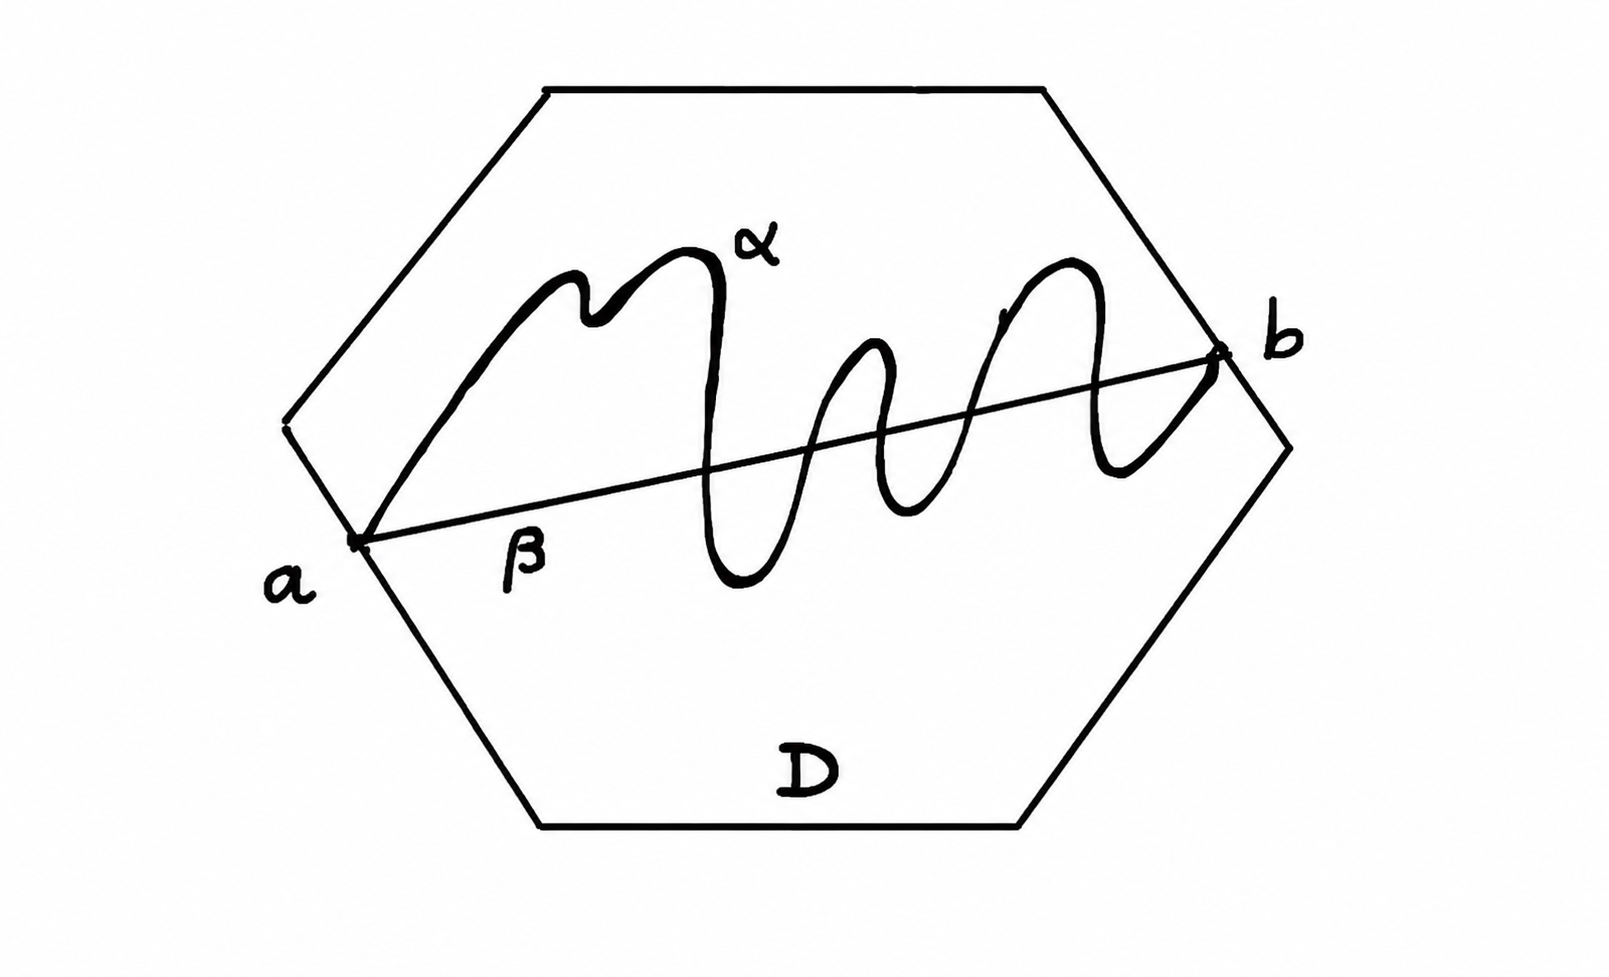
\includegraphics[width=90mm,scale=1]{figs/5.png}
%\end{minipage}
%\vskip .3cm
Par définition, un \emph{circuit} de $(k, \omega)$ (ou encore un $\omega$-circuit de $k$) est une orbite de $\varphi_\omega$ (Noter que toute boucle isolée, tout point isolé est un circuit). On notera $F(k, \omega)$ l'ensemble des circuits de $(k,\omega)$, ils définissent une partition de $E$. 
\vskip .3cm
{\bf 1.5.2}. --- Soit maintenant $(K,\omega)$ un 1-complexe topologique (compact) circularisé et soit $(k,\omega) = \mathcal{C}(K,\omega)$ (cf. 1.4.).

On considère le 1-complexe topologique orienté (i.e. dont chacune des arêtes est munie d'une orientation) réunion disjointe des arcs et des sommets isolés de $K$. On réunit et on recolle ses différentes composantes connexes selon la loi :

Pour tout arc $a$ (avec source) de $K$, soit $\tilde{b}(a)$ le but de $a$ (cf. I.1.2.), $x = b(a)$ le but de $a$ dans $K$, $a' = \omega_x^{-1}(\sigma(a))$ l'arc, on identifie le point $\tilde{b}(a)$ de $a$ avec le point $\tilde{s}(a')$ de $a'$ ($\tilde{s}(a')$ est la source de $a'$, cf. I.1.2.).

%\vskip .3cm
%\begin{minipage}{\linewidth}
%    \centering
%    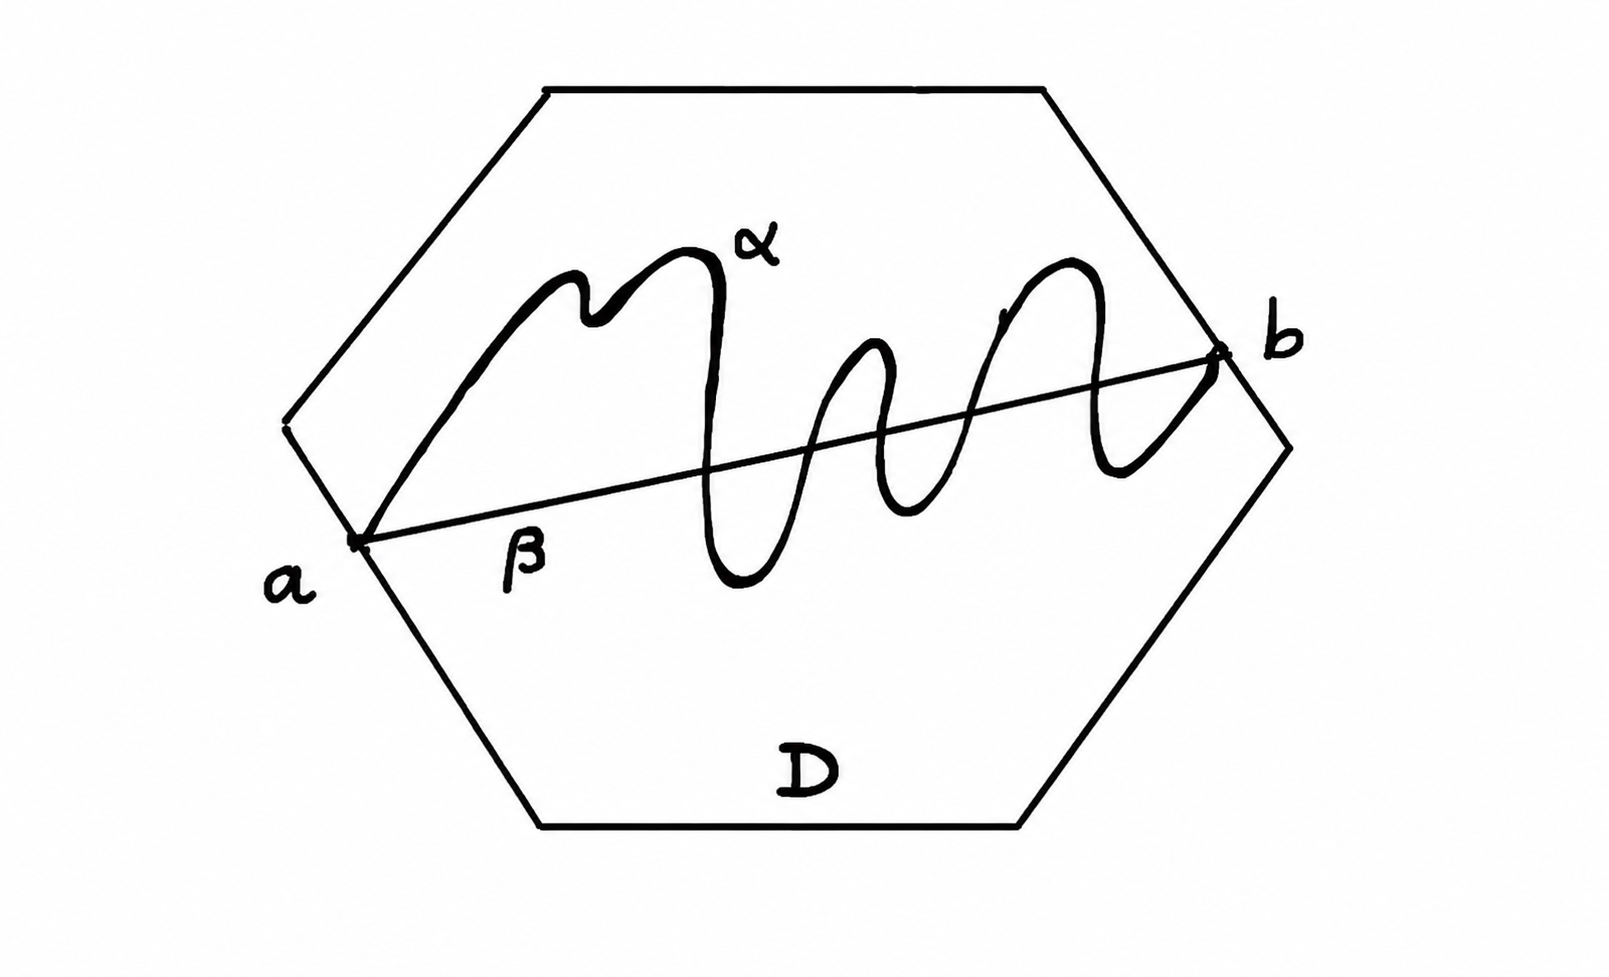
\includegraphics[width=90mm,scale=1]{figs/5.png}
%\end{minipage}
%\vskip .3cm

L'espace quotient ainsi obtenu, muni de la partie finie formée par l'ensemble des points $\tilde{s}(a)$ (où $a$ décrit l'ensemble des arcs avec source de $K$) et des sommets isolés de $K$ est un 1-complexe topologique compact orienté qu'on notera $\Gamma(K,\omega)$ et qu'on appellera \emph{1-complexe topologique des circuits de $(K,\omega)$}.

Il existe une projection canonique de $\Gamma(K,\omega)$ sur $K$, induite par les projections canoniques $P_a$ de $a$ dans $K$ (cf. I.1.2.) (pour tout arc $a$ de $K$).

Par construction, il est clair que l'ensemble des sommets de $\Gamma(K,\omega)$ est constitué par l'ensemble des sommets isolés de $K$ (ce sont aussi des sommets isolés de $\Gamma(K,\omega)$) réuni à un ensemble de sommets de degré 2 (à savoir : les $\tilde{s}(a)$). Par conséquent, à chaque arc $a$ de $K$ correspond (de façon bijective) une arête $a_\Gamma$ de $\Gamma(K,\omega)$ ; à cette arête sont associées deux arcs de $\Gamma(K,\omega)$ : d'une part $a_\Gamma$ munie de l'orientation induite par $a$, d'autre part $a_\Gamma$ munie de l'orientation inverse de celle induite par $a$ ; on en déduit une bijection canonique entre l'ensemble $A_\Gamma$ des arcs de $\Gamma(K,\omega)$ et l'ensemble $A \times \{1,-1\}$ (bijection qui à $a_\Gamma$ munie de l'orientation (resp. orientation inverse) de $a$, associe $(a,1)$ (resp. $(a,-1)$)).

L'ensemble des composantes connexes de $\Gamma(K,\omega)$ sera noté $F(K,\omega)$, il est (de façon évidente, vu les opérations de recollement, et la définition 1.5.1.) en bijection canonique avec $F(k,\omega)$, par l'application qui à toute composante $\gamma$ de $\Gamma(K,\omega)$ associe l'ensemble des arcs de $K$ (ou sommets isolés de $K$) dont $\gamma$ est le recollement.
\vskip .3cm
{\bf 1.5.3}. --- Revenons au cas d'un 1-complexe combinatoire circularisé $(k,\omega)$ ($k = (S,A,B,\sigma,s)$, $S_0$ désignera l'ensemble des sommets isolés de $k$).

On lui associe un 1-complexe combinatoire des circuits de $(k,\omega)$, noté $\gamma(k,\omega)$, qui est, par définition :
\[
\gamma(k,\omega) = (S_0 \amalg A \setminus B, A \times \{1,-1\}, B \times \{1,-1\}, \sigma_\gamma, s_\gamma)
\]
où $\sigma_\gamma$ est l'application de $A \times \{1,-1\}$ dans lui-même définie par :
\[
\forall (a,i) \in A \times \{1,-1\}, \quad \sigma_\gamma(a,i) = (a,-i)
\]
et où $s_\gamma$ est l'application de $(A \setminus B) \times \{1,-1\}$ dans $F(k,\omega)$ définie par :
\[
\forall (a,1) \in (A \setminus B) \times \{1,-1\}, \quad s_\gamma(a,1) = b(a)
\]
(rappelons que $b(a) = s(\sigma(a))$, cf. I.2.1.).
\vskip .3cm
{
Proposition {\bf 1.5.4.} --- \it Si $(K,\omega)$ est un 1-complexe topologique circularisé, et si $c(K)$ est la représentation combinatoire de $K$, il existe un isomorphisme canonique de 1-complexes combinatoires :
\[
c(\Gamma(K,\omega)) = \gamma(c(K),\omega)
\]    
}
\vskip .3cm
Démonstration. --- Comme en 1.5.2., notons $k = c(K)$. Il existe (cf. 1.5.2.) une bijection canonique entre l'ensemble $A_\Gamma$ des arcs de $\Gamma(K,\omega)$ et l'ensemble $A \times \{1,-1\}$ (où $A$ est l'ensemble des arcs de $K$). Il existe également une bijection canonique entre l'ensemble des sommets de $\Gamma(K,\omega)$ et l'ensemble $S_0 \amalg (A \setminus B)$ ($k = (S,A,B,\sigma,s)$ et si $S_0$ désigne l'ensemble des sommets isolés de $K$) (cf. 1.5.2. également). Le couple $b = (\varphi,\psi)$ est l'isomorphisme canonique annoncé entre $c(\Gamma(K,\omega))$ et $\gamma(k,\omega)$.
\vskip .3cm
Remarque. --- une orientation d'un 1-complexe combinatoire $k = (S,A,B,\sigma,\emptyset)$ est la donnée d'une partie $A_0$ de $A$ telle que $A = A_0 \amalg \sigma(A_0)$. Le 1-complexe $\gamma(k,\omega)$ est donc canoniquement orienté par le choix de la partie $A \times \{1\}$ de $A \times \{1,-1\}$. De même l'orientation de $\Gamma(K,\omega)$ induit, de façon naturelle, une orientation de $c(\Gamma(K,\omega))$ ; il est alors clair que l'isomorphisme canonique $b : c(\Gamma(K,\omega)) \simeq \gamma(k,\omega)$, introduit ci-dessus, respecte les orientations.
\vskip .3cm
{\bf 1.5.5}. --- Fonctorialité de $F(k,\omega), \Gamma(K,\omega), F(K,\omega), \gamma(k,\omega)$.

Si $(k,\omega)$ et $(k',\omega')$ sont deux 1-complexes combinatoires circularisés (objets de $kc$), et $b$ un $kc$-isomorphisme de $(k,\omega)$ sur $(k',\omega')$ ($b = (\varphi,\psi)$, cf. 1.3.), l'application est une bijection de l'ensemble $A$ des arcs de $k$ sur l'ensemble $A'$ des arcs de $k'$, qui induit (vu la définition 1.5.1. de $F(k,\omega)$ et $F(k',\omega')$, et le fait que $b$ respecte les circularisations) une bijection $F(b)$ entre $F(k,\omega)$ et $F(k',\omega')$.

De $b$ on déduit également de façon canonique un isomorphisme $\gamma(b)$ de 1-complexes combinatoires orientés entre $\gamma(k,\omega)$ et $\gamma(k',\omega')$, à savoir (si $k = (S,A,B,\sigma,s)$ et si $S_0$ désigne l'ensemble des sommets isolés de $k$) :
\[
\gamma(b) = ((\varphi|_{S_0}) \amalg (\psi|_{A \setminus B}), \psi \times \operatorname{id}_{\{1,-1\}})
\]

Si $(K,\omega)$ et $(K',\omega')$ sont deux 1-complexes topologiques circularisés (objets de $KT$) et $h$ un isomorphisme (de $KT$) entre $(K,\omega)$ et $(K',\omega')$, alors $h$ induit un isomorphisme $\tilde{h}$ du 1-complexe topologique orienté réunion disjointe des arcs et sommets isolés de $K$ sur le 1-complexe topologique orienté réunion disjointe des arcs et sommets isolés de $K'$. Cet $\tilde{h}$ passe au quotient par les opérations de recollement qui permettent de définir $\Gamma(K,\omega)$ et $\Gamma(K',\omega')$, et induit un isomorphisme $\Gamma(h)$ (de 1-complexes topologiques orientés) entre $\Gamma(K,\omega)$ et $\Gamma(K',\omega')$. Ce dernier isomorphisme induit une bijection entre les ensembles de composantes connexes de $\Gamma(K,\omega)$ et $\Gamma(K',\omega')$, bijection qu'on notera $F(h) : F(K,\omega) \cong F(K',\omega')$.

Bien entendu, si $(k,\omega) = c(K,\omega)$ et $(k',\omega') = c(K',\omega')$ 

(cf. 1.4. pour la définition du foncteur $\curvedarrow{c}$), les deux diagrammes suivants sont commutatifs~:
\[\begin{tikzcd}
	{F(K, \omega)} & {F(K',\omega')} \\
	{F(k,\omega)} & {F(k',\omega')}
	\arrow["{F(h)}", from=1-1, to=1-2]
	\arrow["\wr"', from=1-1, to=2-1]
	\arrow["\wr"', from=1-2, to=2-2]
	\arrow["{F(\curvedarrow{a}(h))}", from=2-1, to=2-2]
\end{tikzcd}\]
\[\begin{tikzcd}
	{c(\Gamma(K,\omega))} & {\gamma(k,\omega)} \\
	{c(\Gamma(K',\omega'))} & {\gamma(k',\omega')}
	\arrow["\sim", from=1-1, to=1-2]
	\arrow["{c(\Gamma(h))}"', from=1-1, to=2-1]
	\arrow["{\gamma(\curvedarrow{c}(h))}", from=1-2, to=2-2]
	\arrow["\sim", from=2-1, to=2-2]
\end{tikzcd}\]

%%%%%%%%%%%%%%%%%%%%%%%%%%%%%%%%%%%%
\subsection*{2. La catégorie des plongements comme produit 2-fibré.}
\addcontentsline{toc}{subsection}{2. La catégorie des plongements comme produit 2-fibré}

{
Théorème {\bf 2.1.} --- \it Soient $X$ une surface à bord généralisé orientée (cf. II.1.1.), $K$ un 1-complexe topologique compact contenu dans $\operatorname{int} X$, $\Sigma(X,K)$ la découpe de $X$ suivant $K$ (cf. II.5.4.), $p$ la projection canonique de $\Sigma(X,K)$ sur $X$, et $K'$ le 1-complexe orienté $p^{-1}(K)$. Il existe un isomorphisme canonique de 1-complexes orientés entre $K'$ et $\Gamma(K,\omega)$ (où $\omega$ est la circularisation induite sur $K$ par le plongement $K \hookrightarrow X$, cf. II.4.2.), rendant commutatif le diagramme :
\[
\begin{array}{ccc}
\Theta : K' & \longrightarrow & \Gamma(K,\omega) \\
& \operatorname{p}|_{K'} \searrow & \downarrow q \\
& & K
\end{array}
\]
(où $q$ désigne la projection canonique de $\Gamma(K,\omega)$ sur $K$, cf. 1.5.2.).     
}
\vskip .3cm
{\bf 2.1.1}. --- Quelques précisions :
d'après II.5.4., $p^{-1}(K)$ est une partie du bord généralisé $\partial'\Sigma(X,K)$ ; si on munit l'espace topologique $p^{-1}(K)$ de la partie finie $p^{-1}(S)$ (où $S$ est l'ensemble des sommets de $K$), on obtient un 1-complexe, et c'est celui-là qu'on désigne par $K'$ dans l'énoncé ci-dessus. $K'$ est un 1-complexe orienté car $\Sigma(X,K)$ est une surface à bord généralisé orientée (par l'orientation induite par celle de $X$ : $\operatorname{int}\Sigma(X,K) = (\operatorname{int} X \setminus K)$), ce qui induit, de ce fait, une orientation sur son bord, et donc sur toute arête de $K'$, puisque $K' \subset \partial'(X,K)$.

\paragraph{N.B.} Comme, d'après II.5.5.2., $X$ est l'espace quotient de $\Sigma(X,K)$ par la projection canonique $\Sigma(X,K) \rightarrow X$, il résulte de 2.1. que $X$ est canoniquement homéomorphe à l'espace $\Sigma(X,K) \coprod_{q \circ \Theta} K$, recollement de $\Sigma(X,K)$ et $K$ par l'application $q \circ \Theta : K' \rightarrow K$.
\vskip .3cm
{\bf 2.1.2}. --- Démonstration de 2.1. Comme $K'$ est construit localement au-dessus de chaque $x \in K$ (Rappelons que $K' = \bigcup_{x \in K} \pi(X,K;x)$, cf. II.5.), il suffit, pour chaque $x \in K$, de construire un homéomorphisme orienté $\theta_V$ entre $p^{-1}(V)$ et $q^{-1}(V)$, où $V$ est un voisinage de $x$ dans $K$.

Soit donc $x \in K$, $x$ de degré $n \ge 2$ (le cas $n = 0$ est trivial, et le cas $n = 1$ est un peu particulier et nécessite quelques modifications à la démonstration qu'on donne ci-dessous, modifications laissées au lecteur), et soit $(D,h)$ une carte adaptée au plongement $K \hookrightarrow X$ en $x$ (cf. II.2.3.) ; alors $h$ est un homéomorphisme orienté du couple $(D, D \cap K)$ sur $(\mathbb{B}(0;1), \overline{\text{st}}_n)$. Soient $a_1, a_2, \dots, a_n$ (dans cet ordre circulaire) les $n$ arcs de $K$ issus de $x$, on désignera par $\check{a}_1, \check{a}_2, \dots, \check{a}_n$ leurs projections canoniques respectives dans $K$, et par $p_1, p_2, \dots, p_n$ les points d'intersections respectifs des $\check{a}_i$ ($i = 1, \dots, n$) avec $\partial D$ ; on prend pour voisinage $V$ de $x$ dans $K : V = D \cap K$, donc $V = \bigcup_{i=1}^n [x, p_i]$, chaque segment $[x, p_i]$ étant la partie $D \cap a_i$ de $\check{a}_i$.

\begin{enumerate}
    \item $q^{-1}(V) = \bigcup_{i=1}^n q^{-1}([x, p_i])$, et pour chaque $i = 1, \dots, n$, $q^{-1}([x, p_i])$ est constitué d'une partie $\alpha_i$ de l'arc $a_i$ (à savoir $\alpha_i = \mathbb{P}_i^{-1}([x, p_i])$ où $\mathbb{P}_i$ désigne l'application canonique de $a_i$ dans $K$) et d'une partie $\alpha_i'$ de l'arc $\sigma(a_i)$ (à savoir $\alpha_i' = \mathbb{P}_i'^{-1}([x, p_i])$, où $\mathbb{P}_i'$ désigne l'application canonique de $\sigma(a_i)$ dans $K$), les deux parties $\alpha_{i-1}$ et $\alpha_i'$ étant recollées (vu les opérations de recollement qui définissent $\Gamma(K,\omega)$, cf. 1.5.2.) par la loi :
    
    Le point $\tilde{b}(\sigma(a_i))$ de $\alpha_i'$ (i.e. point but de $\sigma(a_i)$) est identifié au point $\tilde{s}(a_{i-1})$ de $\alpha_{i-1}$ (i.e. point source de $a_{i-1}$), en convenant de poser $\alpha_0 = \alpha_n$, $a_0 = a_n$ ; le point de $\Gamma(K,\omega)$ ainsi obtenu par identification sera noté $x_{i-1}$ (avec la convention $x_0 = x_n$).
    
    Il y a donc exactement $n$ points dans $q^{-1}(V)$ au-dessus de $x$ : $x_1, x_2, \dots, x_n$. Par contre si $y \in [x, p_i]$, il y a au-dessus de $y$, dans $q^{-1}(V)$, exactement deux points $\tilde{y}, \tilde{y}'$ ($\tilde{y} \in \alpha_i, \tilde{y}' \in \alpha_i'$). Il résulte de l'étude ci-dessus que $q^{-1}(V)$ est la réunion disjointe de $n$ composantes connexes $\beta_1, \beta_2, \dots, \beta_n$ où on note $\beta_{i-1} = \alpha_i' \coprod \alpha_{i-1}$ (recollement de $\alpha_i'$ et $\alpha_{i-1}$ avec la convention $\beta_0 = \beta_n$).
    
    \item Examinons maintenant $p^{-1}(D)$, c'est une partie de $\Sigma(X,K)$ canoniquement…
\end{enumerate}

\vskip .3cm
{\bf 2.2}. ---


\vskip .3cm
{\bf 2.3}. ---



%%%%%%%%%%%%%%%%%%%%%%%%%%%%%%%%%%%%
\subsection*{3. Classification à congruence près des plongements de 1-complexes topologiques compacts dans les surfaces à bord généralisé orientées compactes.}
\addcontentsline{toc}{subsection}{3. Classification à congruence près des plongements de 1-complexes topologiques compacts dans les surfaces à bord généralisé orientées compactes}

{\bf 3.1}. --- 

\vskip .3cm
{\bf 3.2}. ---

\vskip .3cm
{\bf 3.3}. ---


\vskip .3cm
{\bf 3.4}. ---



%%%%%%%%%%%%%%%%%%%%%%%%%%%%%%%%%%%%
\subsection*{4. Voisinages tubulaires de 1-complexes.}
\addcontentsline{toc}{subsection}{4. Voisinages tubulaires de 1-complexes}

{\bf 4.1}. --- 

\vskip .3cm
{\bf 4.2}. --- Voisinage tubulaire associé à un plongement.

\vskip .3cm
{\bf 4.3}. ---

\vskip .3cm
{\bf 4.4}. ---

\vskip .3cm
{\bf 4.5}. ---


%%%%%%%%%%%%%%%%%%%%%%%%%%%%%%%%%%%%
\subsection*{5. Plongement cellulaires.}
\addcontentsline{toc}{subsection}{5. Plongement cellulaires}

{\bf 5.1}. --- 

\vskip .3cm
{\bf 5.2}. ---

\vskip .3cm
{\bf 5.3}. ---

\vskip .3cm
{\bf 5.4}. ---

\vskip .3cm
{\bf 5.5}. ---

%%%%%%%%%%%%%%%%%%%%%%%%%%%%%%%%%%%%
\subsection*{6. Plongements minimaux.}
\addcontentsline{toc}{subsection}{6. Plongements minimaux}

{\bf 6.1}. --- 

\vskip .3cm
{\bf 6.2}. ---

\vskip .3cm
{\bf 6.3}. ---


%%%%%%%%%%%%%%%%%%%%%%%%%%%%%%%%%%%%
\subsection*{7. Quelques remarques sur le cas des plongements dans les surfaces à bord non orientées (pouvant être non orientables).}
\addcontentsline{toc}{subsection}{7. Quelques remarques sur le cas des plongements dans les surfaces à bord non orientées (pouvant être non orientables)}

On peut introduire la notion de voisinage tubulaire standard non orienté (et éventuellement non orientable) d'un $1$-complexe $K$. Ces voisinages tubulaires sont classifiés pour la donnée d'un revêtement étale à deux feuillets $\tilde{K}$ de $K$ et d'une circularisation $\tilde{\omega}$ ``antisymétrique'' de $\tilde{K}$ (i.e.~: $\tau_* \tilde{\omega} = \tilde{\omega}^{-1}$, où $\tau$ est l'automorphisme involutif et sans point fixe du revêtement $\widetilde{K} \to K$). On peut aussi classifier ces voisinages tubulaires par des couples $(\omega, \xi)$ où $\omega$ est une circularisation de $K$, et $\xi$ une classe de cohomologie de $\mathrm{H}^1(K; \mathbf{Z}/2\mathbf{Z})$. On obtient alors un théorème de classification à congruence près (non orientée) des plongements dans les surfaces non orientées, théorème d'énoncé beaucoup plus technique que {\bf 3.4.3}. L'essentiel des résultats est donné dans [63].


% End
